\documentclass{article}
\usepackage[utf8]{inputenc}
\usepackage[margin=1.0in]{geometry}
\usepackage{amsmath}
\usepackage{mathtools}
\usepackage{amsfonts}
\usepackage{amssymb}
\usepackage{changepage}
\usepackage{setspace}
\usepackage{verbatim}
\usepackage{xhfill}
\usepackage{sectsty}
\usepackage{enumitem}

\usepackage{color}
\newcommand{\katznote}[1]{ {\textcolor{magenta}    { ***Dan:      #1 }}}

\sectionfont{\fontsize{10}{15}\selectfont}
\renewcommand{\arraystretch}{1.5}
\setlist{noitemsep}

\begin{document}

\begin{center}
    \textbf{2018 CSE Fellowship Application - Research proposal}
\hfill
\textbf{Joshua Vita}
\end{center}
\noindent\hrulefill

\bigskip

\katznote{this dives in, expecting reviewers to understand what comptational material science is, what potentials are, and what empirical potentials are.  I would start with a more introductory paragraph or at least a few sentences about this, since reviewers will likely be from multiple fields.  Also explain what you are predicting wrt `predictive accuracy'} In computational materials science, empirical potentials are a fundamental element of multiscale modeling that allow for a balance between predictive accuracy and computational cost that is unattainable using typical first-principles techniques. Through the use of empirical potentials, molecular dynamics simulations have been able to access \katznote{how to simulations access anything?} system sizes on the order of $10^6$ - $10^9$ atoms and timescales of nano- to micro seconds (or even longer), impacting a wide array of fields, from materials science and physics to chemistry and even biology. The ability to develop accurate, robust potentials without sacrificing significant amounts of human effort is thus an inherently wide-reaching challenge. Our \katznote{maybe `my'?} current work aims to build a massively parallel optimization engine that leverages not only the petascale computing powers available to us, but also the rapidly-growing materials databases that are being produced by the community.

\bigskip

Standard methods of developing empirical potentials (even taking into account popular potential fitting software \cite{potfit}) can in many ways be jokingly \katznote{instead of `can in many ways be jokingly', maybe `are sometimes'} described as a type of ``black magic" since they require a large amount of intuition and fine-tuning by trained professionals. The biggest challenge in this technique is selecting an appropriate set of atomic configurations to be used to fit the potential in order to accurately model the physical and chemical processes of interest (we will refer to the method of choosing a set of configurations as `database optimization'). Due to the necessary cycle of fitting, testing, and retesting a potential, the production of a `good' interatomic potential can take months or even years of work by experts in the field.

Previous work in our group developed a new approach to database optimization that utilizes Bayesian inference \cite{baye} and Markov Chain Monte Carlo methods to iteratively select the optimal subset of a materials database for use in potential fitting \cite{dbopt}. This method, outlined in Figure \ref{fig:workflow}, effectively reduces the need for human intervention and guesswork associated with the fitting process, potentially condensing months or years of active research into a simple matter of computer walltime. As a proof-of-concept, our group used this new algorithm to augment an existing titanium potential to include titanium-oxygen interactions, creating a useful binary alloy potential \cite{tio}. \katznote{this is good, but there's too much us, and not enough I - particular going forward in terms of what you are actually going to do.}

\begin{figure}[h!]
  \centering
  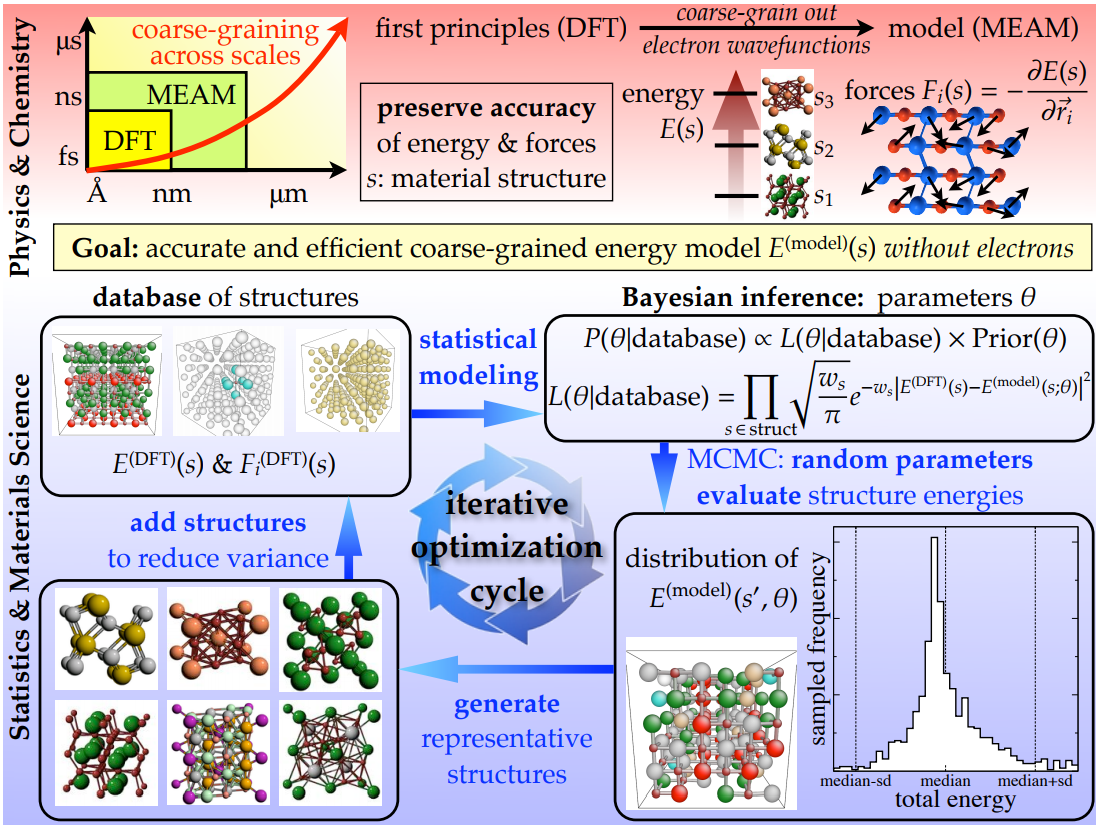
\includegraphics[width=0.65\linewidth]{workflow.png}
  \caption{\textit{A general overview of the workflow demonstrated by previous work in our group \cite{dbopt}. Integral to the scalability of this process, and the purpose of the currently proposed work, is to design a massively parallel evaluation engine for rapid evaluation of energies and forces of all structures in the database.}}
  \label{fig:workflow}
\end{figure}

At the center of this algorithm, or related algorithms that we \katznote{I?} could develop in the future, needs to be a massively parallel evaluation engine that takes a list of structures (atomic positions and chemistries), and a large vector of parameters for the empirical potential, and evaluates the energies and forces of each structure for each parameter set. As more parameters and structures are included into the database, through prediction of new structures using both \textit{ab initio} techniques like density-functional theory and empirical parameter optimization, the need for a massively parallel approach becomes readily apparent. For example, if we consider

\begin{itemize}
    \item $\bf{10^6}$ potential parameters, which is on the order needed for Bayesian sampling, applied to
    \item $\bf{10^3}$ atomic configurations
\end{itemize}

\noindent Then while each individual calculation may require mere milliseconds to complete, we have approximately $~10^9$ computations requiring multiple terabytes of data being used simultaneously. While these calculations are, fortunately, embarrassingly parallel and can be considered \katznote{executed} with a master-worker approach, advanced algorithms are required to properly handle the parallel workflow and large amounts of simultaneous data. Nevertheless, if we are able to achieve these larger scales, the structural and energy landscapes of an empirical potential could be fully analyzed to produce accurate, predictive, and transferable empirical potentials. \katznote{what would this enable?} The purpose of my current work is to design and implement such a massively parallel evaluation, to be used as the framework through which to deploy the new algorithm developed by our group.

\bigskip

This task has effectively transformed \katznote{effectively transforms} a purely materials science problem (potential fitting) into an interdisciplinary challenge requiring expertise and collaboration in the fields of high performance computing and software development for massively parallel applications. The goal of achieving petascale parallelization is on its own something that has been rarely achieved in computational materials science in general and remains largely untouched in terms of potential fitting in particular. Success would be a meaningful step in the field of materials modeling towards proper utilization of cutting-edge supercomputing capabilities.

Not only would this work be significant because of how it would help push potential fitting onto supercomputing platforms, but also because of how much it could lower the barrier to entry for exploration into new materials systems via computational methods. As was mentioned previously, development of new interatomic potentials (the first step towards analyzing a new materials system) can take anywhere from months to years and requires dedicated efforts by multiple experts. Because of this, it can be difficult for researchers to commit to the undertaking of working with a system that hasn't already been modeled by an existing empirical potential. Since materials research is largely driven by a desire to discover new materials, this barrier associated with developing new empirical potentials has a strong impact on scientific progress in the field. The possibility for rapid development of potentials, as is the goal in my work, would encourage investigation into newer and more complex systems, which would in turn influence many fields in science and engineering. \katznote{this is good - maybe some of it, or something similar could be used at the start as well?}

\bigskip

Beyond its influence \katznote{impact} in the scientific community, I also see this work as being \katznote{drop `being'} a critical step in my professional development. Ever since the early years of my college career, I've been \katznote{drop `been'} focused on advancing my skills in software development and knowledge of mathematics, with the broad goal of someday being able to apply them towards real-world scientific problems. While my interests have always been intimately tied to the questions being asked by materials scientists, I also love the experience of getting to build new, innovative, and powerful pieces of software in order to answer those questions. To me, my work here at the University of Illinois feels like the perfect means by which I can begin truly contributing to the scientific community.

In addition to being a way of providing a useful tool to my community, this work has also introduced me to the burgeoning field of research software engineering; a subset of software development that is specifically focused on supporting the growth of scientific software applications in research. This society is populated by many people like myself who are driven to solve problems from physics, chemistry, and engineering, but who are using programming as their tool of choice. My goal over the next few years is to prepare myself to be able to contribute to large-scale collaborative efforts in scientific software development. I see my current work as an opportunity not only to refine my technical skills (in terms of coding and good software development practices), but also as a chance to gain more experience in collaborative development and software deployment on high performance computers.

Given the inherently interdisciplinary nature of my work and its potential for wide-reaching impacts, I think that it would \katznote{will} serve as an excellent example of the type of work being done by the CSE community here on campus. Not only does it provide a clear link between materials science and petascale computing, but it also could fundamentally change how researchers broach the task of exploring a whole class of materials systems. On a more personal level, working on this project is the perfect conduit through which to further my goals of being able to contribute to society as a research software engineer. Thank you for taking the time to consider my proposal; I look forward to continuing to contribute to the CSE community and to seeing all of the impressive work being done by next year's CSE Fellows.

\bibliography{bibliography}
\bibliographystyle{plain}

\end{document}